
\documentclass[../main.tex]{subfiles}

\begin{document}

\chapquote{To become good at anything you have to know how to apply basic principles. To become great at it, you have to know when to violate those principles.}{Garry Kasparov}
\chapter{Background}
This chapter will introduce some of the basic concepts involved in \glspl{ann}, \glspl{cnn}, and transfer learning required to understand this report.
Readers familiar with this subject matter should feel free to skip this chapter and resume at \cref{chap:data_synthesis}.

\section{Supervised learning}
At its core, the purpose of an \gls{ann} is to infer a function that maps some input to some output, based on sample input-output pairs.
In machine learning, we call this a \emph{supervised learning} task, and there are a great number of machine learning models (not only \glspl{ann}) that have been developed for this task.
We shall briefly examine the two main disciplines within supervised learning: \emph{regression} and \emph{classification}.

\subsection{Regression}
\label{sec:regression}
A regression model captures the relationship between multiple input variables and one output variable. 
As such, it can be defined a mathematical function of the form $f:\mathbb{R}^n\rightarrow \mathbb{R}$ given by
\begin{equation}
    \label{eq:reg_model}
    f(\vx) = \hat{y} = y + \epsilon
\end{equation}
that models the relationship between a $n$-dimensional feature vector $\vx \in \mathbb{R}^n$ of independent (\emph{input}) variables and the dependent (\emph{output}) variable $y \in \mathbb{R}$. 
Given a particular $\vx$, the model will produce a \emph{prediction} for $y$ which we shall denote $\hat{y}$.
Here, the additive error term $\epsilon$ represents the discrepancy between $y$ and $\hat{y}$, i.e. the difference between the predicted and observed output.

A labelled dataset for a regression task consists of $m$ tuples of the form
$\langle \vx_i, y_i\rangle$
for $i=1,\dots,m$.
For each feature vector $\vx_i$ (a row vector), the corresponding $y_i$ represents the observed output, or \emph{label} \cite{burkov2019}.
We use the vector
\begin{equation}
    \label{eq:sup_learn_target}
    \vy = \begin{bmatrix}
        y_1 & y_2 & \cdots & y_m
    \end{bmatrix}^\top
\end{equation}
to denote all the labelled outputs in the dataset, and the $m \times n$ matrix
\begin{equation}
    \label{eq:sup_learn_input_matrix}
    \mX = \begin{bmatrix}
        \vx_1 & \vx_2 & \cdots & \vx_m
    \end{bmatrix}^\top
\end{equation}
for representing the corresponding feature vectors.

\subsection{Classification}
\label{sec:background_classification}
Classification is a task that finds greater applicability within this project.
As the name implies, a classification model tries to determine which category each input sample belongs to from a predefined set of classes $\sC$.
To ease notation, we shall let $\sC=\{1, 2, \dots, C\}$ where $C$ is the total number of classes.
In practical terms, the elements in $\sC$ could represent any type of mathematical or non-mathematical object, and in that case we only require a one-to-one mapping from those objects to $\sC$.
Furthermore, in the context of this report, each input sample can only belong to one class, and we will interpret the output of the model to represent the probabilities of the input sample belonging to each of the classes $\sC$.
Therefore, a classification model is represented by a vector-valued function
$\vf : \mathbb{R}^n \rightarrow [0,1]^{\abs{\sC}}$
instead of a scalar function as in \cref{eq:reg_model}, namely
\begin{equation}
    \label{eq:cla_model}
    \vf(\vx) = \vyhat = \vy + \vec{\epsilon}.
\end{equation}
Here, $\vf(\vx)$ actually represents a \gls{pmf} where the $i$\textsuperscript{th} component $\hat{y}_i$ of the output vector $\vyhat$ represents the probability that the input sample $\vx$ belongs to the class $i\in \sC$.
It follows that
\begin{equation}
    \label{eq:pmf}
    \sum_{i=1}^{\abs{\sC}} \hat{y}_i = 1.
\end{equation}

The observed output $\vy$ is a row vector that uses a \gls{ohe} to represent the sample's class. 
This means that for a given class $c \in \sC$, the components of $\vy$ are given by
\begin{equation*}
    y_i = \begin{cases}
        1 & i=c \\
        0 & \text{otherwise}
    \end{cases},
\end{equation*}
which retains the property described in \cref{eq:pmf}.
Since $\vf$ represents a \gls{pmf}, the one-hot encoded vector essentially states that the probability of class $c$ is 100\% and all other classes have a probability of 0\%.
Notice that our outputs are now the vectors $\vy_i$ instead of the scalars $y_i$ in the regression task.
Hence a labelled classification dataset will consist of $m$ tuples of the form $\langle \vx_i,\vy_i \rangle$, meaning that instead of the vector $\vy$ from \cref{sec:background_classification}, we must use a matrix
\begin{equation}
    \mY = \begin{bmatrix}
        \vy_1 & \vy_2 & \cdots & \vy_m
    \end{bmatrix}^\top
\end{equation}
to denote the targets.
Each row in $\mY$ represents the one-hot encoded class label for that sample. 
The input matrix $\mX$ remains as defined in \cref{eq:sup_learn_input_matrix}.

\section{\Glsentrylongpl{ann}}
\label{sec:ann}
\Glspl{ann} take inspiration from the human brain and can be regarded as a set of interconnected neurons. 
More formally, an \gls{ann} is a directed graph of $n$ neurons (referred to as \emph{nodes} or \emph{units}) with weighted edges (\emph{links}).
Each link connecting two units $i$ and $j$ is directed and associated with a real-valued weight $w_{i,j}$. 

A particular unit $i$'s \emph{excitation}, denoted $z_i$, is calculated as the weighted sum
\begin{equation}
    \label{eq:ann_excitation}
    z_i = \sum_{j=1}^n{w_{j,i} a_j} + b_i
\end{equation}
where $a_j \in \mathbb{R}$ is another unit $j$'s \emph{activation} and $b_i \in \mathbb{R}$ is the $i$\textsuperscript{th} unit's \emph{bias}.
In this model, if there exists no link between unit $i$ and a particular $j$ then simply $w_{i,j}=0$ and therefore $j$ will not contribute to $i$'s excitation. 
\Cref{fig:ann} gives an example how such a network could look like.
\begin{figure}
    \centering
    \begin{tikzpicture}
        [
            neuron/.style = {draw, circle, minimum size=25pt, inner sep=0pt, outer sep=0pt},
        ]
        \node [neuron] (n1) at (0,0) {$a_1$};
        \node [neuron] (n2) [below left=1cm and .5cm of n1] {$a_2$};
        \node [neuron] (n3) [below right=1cm and .5cm of n2] {$a_3$};
        \node [neuron] (n4) [right=1cm of n3] {$a_4$};
        \node [neuron] (n5) [above right=1cm and .5cm of n4] {$a_5$};
        \node [neuron] (n6) [above left=1cm and .5cm of n5] {$a_6$};
        \node (x1) at (-3, 0 |- n1) {$x_1$};
        \node (x2) at (-3, 0 |- n2) {$x_2$};
        \node (x3) at (-3, 0 |- n3) {$x_3$};
        \node (y1) at (5, 0 |- n6) {$\yhat_1$};
        \node (y2) at (5, 0 |- n5) {$\yhat_2$};
        \draw[->] (x1) -- (n1);
        \draw[->] (x2) -- (n2);
        \draw[->] (x3) -- (n3);
        \draw[->] (n6) -- (y1);
        \draw[->] (n5) -- (y2);
        \draw[->] (n1) -- (n6) node[midway,above] {$w_{1,6}$};
        \draw[->] (n1) -- (n4) node[pos=.8,fill=white] {$w_{1,4}$};
        \draw[->] (n2) -- (n6) node[near start,fill=white] {$w_{2,6}$};
        \draw[->] (n5) -- (n4) node[midway,fill=white] {$w_{5,4}$};
        \draw[->] (n6) -- (n5) node[midway,fill=white] {$w_{6,5}$};
        \draw[->] (n3) -- (n6) node[near start,fill=white] {$w_{3,6}$};
        \draw[->] (n4) -- (n6) node[midway,fill=white] {$w_{4,6}$};
        \node (b1) [above of=n1] {$b_1=0$};
        \node (b2) [above of=n2] {$b_2=0$};
        \node (b3) [below of=n3] {$b_3=0$};
        \node (b4) [below of=n4] {$b_4$};
        \node (b5) [above of=n5] {$b_5$};
        \node (b6) [above of=n6] {$b_6$};
        \draw[->] (b1) -- (n1);
        \draw[->] (b2) -- (n2);
        \draw[->] (b3) -- (n3);
        \draw[->] (b4) -- (n4);
        \draw[->] (b5) -- (n5);
        \draw[->] (b6) -- (n6);
    \end{tikzpicture}
    \caption[An \glsentrylong{ann} with six neurons that could be used to decide a classification problem.]{An \glsentrylong{ann} with six neurons that could be used to decide a classification problem. The inputs $x_1,x_2,x_3$ are set as the activations of the first three units (thus $b_1,b_2,b_3$ have no effect) and the outputs $\yhat_1,\yhat_2$ are the activations received from the final two units. Only some weights are shown in the diagram.}
    \label{fig:ann}
\end{figure}

The unit $i$'s activation is its excitation applied to a non-linear \emph{activation function}, $g: \mathbb{R} \rightarrow \mathbb{R}$. We have
\begin{equation}
    \label{eq:ann_activation}
    a_i = g\left(z_i\right) = g\left(\sum_{j=1}^n{w_{j,i} a_j} + b_i\right).
\end{equation}

\paragraph{Activation functions}
In its original form in \citeyear{mcculloch1943}, \citeauthor{mcculloch1943} defined the neuron as having only binary activation \cite*{mcculloch1943}. 
This means that in our model from \cref{eq:ann_activation}, we would require $a_i \in \{0, 1\}$ and hence an activation function of the form $g_\text{step}: \mathbb{R} \rightarrow \{0, 1\}$ like the Heaviside step function%
\footnote{In fact, \citeauthor{mcculloch1943} defined the activation to be zero when $x<\theta$ for a threshold parameter $\theta \in \mathbb{R}$ and one otherwise, but in our model the bias term $b_i$ acts as the threshold.}
\begin{equation*}
    \label{eq:step_activation}
    g_\text{step}(x) = \begin{cases} 
        0 & x < 0 \\
        1 & x \geq 0
    \end{cases}.
\end{equation*}

Commonly used activation functions in modern neural networks include the sigmoid
\begin{equation*}
    \label{eq:sigmoid}
    g_\text{sig}(x) = \frac{1}{1 + e^{-x}}
\end{equation*}
and the \gls{relu} \cite{glorot2011}
\begin{equation}
    g_\text{ReLU} = \begin{cases}
        0 & x < 0 \\
        x & x \geq 0
    \end{cases}
\end{equation}
which are depicted in \cref{fig:activation_functions}.
\begin{figure}
    \centering
    \begin{subfigure}{.45\textwidth}
        \centering
        \begin{tikzpicture}
            \begin{axis}[
                x=0.75cm,
                y=3cm,
                axis lines=center,
                xlabel={$x$}, xlabel style={anchor=west},
                ylabel={$g_\text{sig}(x)$}, ylabel style={anchor=south},
                ymin=0, ymax=1,
                xmin=-3, xmax=3,
                enlarge x limits,
                enlarge y limits = upper,
                samples=100,
                xtick={-3,...,3},
                ytick={0, 0.5, 1},
                extra x ticks=0
            ]
                \addplot[black] {1 / (1 + exp(-x))};
            \end{axis}
        \end{tikzpicture}
        \caption{Sigmoid}
        \label{fig:activation_functions_sigmoid}
    \end{subfigure}
    \hspace*{\fill}
    \begin{subfigure}{.45\textwidth}
        \centering
        \begin{tikzpicture}
            \begin{axis}[
                x=2.25cm,
                y=3cm,
                axis lines=center,
                xlabel={$x$}, xlabel style={anchor=west},
                ylabel={$g_{\text{ReLU}}(x)$}, ylabel style={anchor=south},
                ymin=0, ymax=1,
                xmin=-1, xmax=1,
                enlarge x limits,
                enlarge y limits = upper,
                samples=100,
                xtick={-1, -0.5, 0, 0.5, 1},
                ytick={0, 0.5, 1},
                extra x ticks=0
            ]
                \addplot[black][domain=0:1] {x};
                \addplot[black][domain=-1:0] {0};
            \end{axis}
        \end{tikzpicture}
        \caption{\Glsentrylong{relu}}
        \label{fig:activation_functions_relu}
    \end{subfigure}
    \caption{Plots of the the two most common activation functions.}
    \label{fig:activation_functions}
\end{figure}
Unlike $g_\text{step}$, the range of these these activation functions is the real numbers, and the functions themselves are differentiable which is an advantage for being able to use gradient descent to optimise the weights \cite[729]{russell2010}.

Rectified units do not suffer from the so-called \emph{vanishing gradient effect} \cite{glorot2011}.
This phenomenon occurs with sigmoid activation functions when they reach high saturation, i.e. when the input is significantly far from zero such that the gradient is almost horizontal (see \cref{fig:activation_functions_sigmoid}), and is especially prevelant in deep neural networks\footnote{Deep neural networks are \glspl{ann} with many layers.}.
As a result, the \gls{relu} activation function (or variants thereof) are the most popular choice nowadays.
Furthermore, the computational cost of the function itself as well as its gradient is cheap.

\subsection{Feedforward neural networks}
Our definition of \glspl{ann} is so far still very general and makes virtually no restrictions on the graph of the network.
It turns out that it is difficult to propagate activations between neurons when they exhibit cycles, as is the case with the last three units in \cref{fig:ann}.
Thus we impose a constraint that the nodes of the network are not allowed to form cycles, and as a result the network becomes a \gls{dag}.
This class of \glspl{ann} are referred to as \emph{feedforward neural networks}.

\subsubsection{\Glsentrylong{slp}}
The most basic type of feedforward neural network is the \gls{slp}.
It consists of $n_0$ input units that are directly connected to $n_1$ output units, as illustrated in \cref{fig:slp}.
\begin{figure}
    \centering
    \begin{tikzpicture}
        [
            neuron/.style = {draw, circle, minimum size=25pt, inner sep=0pt, outer sep=0pt},
        ]
        \node [neuron] (n1) at (0,0) {$\yhat_1$};
        \node [neuron] (n2) [below=1.5cm of n1] {$\yhat_2$};
        \node [neuron] (n3) [below=1.5cm of n2] {$\yhat_3$};
        \node [neuron] (x1) [below left=.75cm and 2cm of n1] {$x_1$};
        \node [neuron] (x2) [below left=.75cm and 2cm of n2] {$x_2$};
        \draw[->] (x1) -- (n1);
        \draw[->] (x1) -- (n2);
        \draw[->] (x1) -- (n3);
        \draw[->] (x2) -- (n1);
        \draw[->] (x2) -- (n2);
        \draw[->] (x2) -- (n3);
        \node (b1) [above of=n1] {$b_1$};
        \node (b2) [above of=n2] {$b_2$};
        \node (b3) [above of=n3] {$b_3$};
        \draw[->] (b1) -- (n1);
        \draw[->] (b2) -- (n2);
        \draw[->] (b3) -- (n3);
    \end{tikzpicture}
    \caption{A \acs{slp} with two inputs and three outputs.}
    \label{fig:slp}
\end{figure}
There are no connections between input units, and no connections between output units.
Likewise, there are no connections from output units to input units. 
The only connections in the network originate from input units and feed to output units. 
In fact, that is where the term \emph{feedforward} arises: the network exhibits neither backwards nor intra-layer connections.
The connections themselves are of course weighted as in any \gls{ann}.
Due to the unidirectional nature of the links, we can continue to use the notation $w_{i,j}$ to denote weights, but now $i$ refers to the input unit and $j$ refers to the output unit.

From \cref{eq:ann_activation}, we can compute the values of the three output units in \cref{fig:slp} as
\begin{equation}
    \label{eq:slp_simple}
    \yhat_j = g\left(\sum_{i=1}^n{w_{i,j} x_i} + b_j\right)
\end{equation}
for $j=1,2,3$.
Mathematically, a \gls{slp} is represented by a function $\vf:\R^{n_0}\to \R^{n_1}$ that maps an input vector $\vx \in \R^{n_0}$ to an output vector $\vyhat \in \R^{n_1}$.
Let us use the $n_0 \times n_1$ matrix $\mW$ to contain all weights such that
\begin{equation*}
    \mW = \begin{bmatrix}
        w_{1,1} & w_{1,2} & \cdots & w_{1,n_1} \\ 
        w_{2,1} & w_{2,2} & \cdots & w_{2,n_1} \\ 
        \vdots & \vdots & \ddots & \vdots \\ 
        w_{n_0,1} & w_{n_0,2} & \cdots & w_{n_0,n_1} \\ 
    \end{bmatrix}.
\end{equation*}
and the vector
\begin{equation*}
    \vb = \begin{bmatrix}
        b_1,b_2,\dots,b_{n_1}
    \end{bmatrix}
\end{equation*}
to represent the biases.
Since the output vector $\vyhat$ is simply the concatenation of the output units, the summation in \cref{eq:slp_simple} we finally define the function of a \gls{slp} as
\begin{equation}
    \label{eq:slp}
    \vf_{\mW,\vb}(\vx) = \vyhat = \vg\left(
        \vw^\top \vx + \vb
    \right)
\end{equation}
where $\vg(\cdot)$ applies the activation function $g$ pointwise.
The process of computing the activations of the output units given the input units is often called \emph{forward propagation} or \emph{forward pass} \cite{burkov2019}.

\subsubsection{\Glsentrylong{mlp}}
As the name implies, a \gls{mlp} simply stacks multiple \glspl{slp} on top of each other, such that each layer's outputs are connected to the next layer's inputs (except for the final layer, where the outputs represent $\vyhat$).
A \gls{mlp} with $L$ layers can be expressed mathematically by composing $L$ \glspl{slp} $\vf_1,\vf_2,\dots,\vf_L$:
\begin{equation}
    \label{eq:mlp}
    \vf(\vx) = (\vf_1 \circ \vf_2 \circ \dots \circ \vf_L)(\vx).
\end{equation}

Each \gls{slp} inside the \gls{mlp} is constitutes a logical module of the \gls{mlp} which we call a \emph{layer}.
Due to the fact that each layer has its own weights $\mW$ and biases $\vb$, we will use the parenthesised superscript notation $\mW^{(l)}$ and $\vb^{(l)}$ to denote the weights and biases in the $l$\textsuperscript{th} layer.
Further, the notation $b_j^{(l)}$ refers to the $j$\textsuperscript{th} unit's bias in layer $l$, and $w_{i,j}^{(l)}$ is the weight of the connection from unit $i$ in layer $l-1$ to unit $j$ in layer $l$.
This notation follows \textcite{goodfellow2016} and is customary in describing neural networks
We shall use $n_0,n_1,\dots,n_L$ to describe the number of units in each layer.
Layer zero is considered the \emph{input layer}, meaning that $n_0$ must be equal to the dimensionality of $\vx$. 
The layers $1, 2, \dots, L-1$ are the \emph{hidden layers} because they are not directly connected to the input or output units.
Finally, we refer to layer $L$ as the \emph{output layer}, since its units represent the prediction $\vyhat$, and so $n_L$ must be equal to the dimensionality of $\vyhat$. 
\Cref{fig:mlp} gives an example of a \gls{mlp} architecture.
\begin{figure}
    \centering
    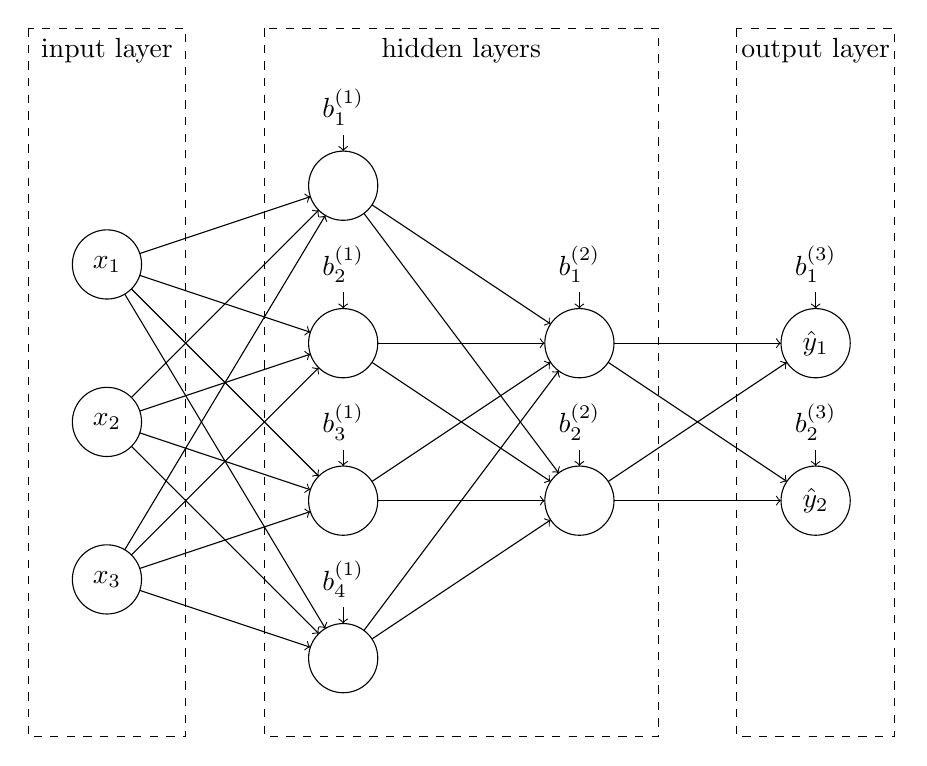
\begin{tikzpicture}
        [
            neuron/.style = {draw, circle, minimum size=25pt, inner sep=0pt, outer sep=0pt},
        ]
        \node [neuron] (x1) at (0,0) {$x_1$};
        \node [neuron] (x2) at (0,-2) {$x_2$};
        \node [neuron] (x3) at (0,-4) {$x_3$};
        \node [neuron] (h11) at (3,1) {};
        \node [neuron] (h12) at (3,-1) {};
        \node [neuron] (h13) at (3,-3) {};
        \node [neuron] (h14) at (3,-5) {};
        \node [neuron] (h21) at (6,-1) {};
        \node [neuron] (h22) at (6,-3) {};
        \node [neuron] (y1) at (9, -1) {$\hat{y}_1$};
        \node [neuron] (y2) at (9, -3) {$\hat{y}_2$};
        \node (b11) at (3, 2) {$b^{(1)}_1$};
        \node (b12) at (3, 0) {$b^{(1)}_2$};
        \node (b13) at (3, -2) {$b^{(1)}_3$};
        \node (b14) at (3, -4) {$b^{(1)}_4$};
        \node (b21) at (6, 0) {$b^{(2)}_1$};
        \node (b22) at (6, -2) {$b^{(2)}_2$};
        \node (b31) at (9, 0) {$b^{(3)}_1$};
        \node (b32) at (9, -2) {$b^{(3)}_2$};
        \draw[->] (x1) -- (h11);
        \draw[->] (x1) -- (h12);
        \draw[->] (x1) -- (h13);
        \draw[->] (x1) -- (h14);
        \draw[->] (x2) -- (h11);
        \draw[->] (x2) -- (h12);
        \draw[->] (x2) -- (h13);
        \draw[->] (x2) -- (h14);
        \draw[->] (x3) -- (h11);
        \draw[->] (x3) -- (h12);
        \draw[->] (x3) -- (h13);
        \draw[->] (x3) -- (h14);
        \draw[->] (h11) -- (h21);
        \draw[->] (h11) -- (h22);
        \draw[->] (h12) -- (h21);
        \draw[->] (h12) -- (h22);
        \draw[->] (h13) -- (h21);
        \draw[->] (h13) -- (h22);
        \draw[->] (h14) -- (h21);
        \draw[->] (h14) -- (h22);
        \draw[->] (b11) -- (h11);
        \draw[->] (b12) -- (h12);
        \draw[->] (b13) -- (h13);
        \draw[->] (b14) -- (h14);
        \draw[->] (b21) -- (h21);
        \draw[->] (b22) -- (h22);
        \draw[->] (b31) -- (y1);
        \draw[->] (b32) -- (y2);
        \draw[->] (h21) -- (y1);
        \draw[->] (h22) -- (y1);
        \draw[->] (h21) -- (y2);
        \draw[->] (h22) -- (y2);
        \draw[dashed] (-1,3) rectangle (1,-6);
        \draw[dashed] (2,3) rectangle (7,-6);
        \draw[dashed] (8,3) rectangle (10,-6);
        \node[below] (input) at (0,3) {input layer};
        \node[below] (hidden) at (4.5,3) {hidden layers};
        \node[below] (output) at (9,3) {output layer};
    \end{tikzpicture}
    \caption{A \acs{mlp} with three inputs, two hidden layers, and two outputs.}
    \label{fig:mlp}
\end{figure}
It can clearly be seen that since \glspl{mlp} are simply nested \glspl{slp}, they still form \glspl{dag} and thus are feedforward networks.
In fact, such networks are usually \emph{fully-connected feedforward networks} because all units from a particular layer connect to all units from the previous layer.

\subsection{Backpropagation}
\emph{Training} with regard to neural networks refers to the process of altering a network's weights and biases with the goal of achieving an optimal configuration that reduces the error of the predictions, i.e. how far they are `off'. 
This is how the network facilitates \emph{learning} the input-output function from \cref{eq:reg_model} that we introduced at the very beginning of this chapter in the context of supervised learning.

Backpropagation with gradient descent is an iterative algorithm for training neural networks that, provided a suitable learning rate $\alpha$, is guaranteed to converge to a \emph{local minimum}.
The main idea is as follows:
\begin{enumerate}
    \item Calculate the derivative of the loss function with respect to the current trainable parameters $\vp$ (weights and biases) as
        $\vec{\Delta p} = \frac{\delta L}{\delta \vp}\left(\vp\right)$.
    \item Take a step in the negative direction of this gradient, i.e. update the trainable parameters $\vp \leftarrow \vp - \alpha \vec{\Delta p}$ where $\alpha \in \R$ is the learning rate.
    \item Repeat steps 1 and 2 until a predefined convergence criterion is met.
\end{enumerate}
\Cref{fig:gradient_descent_local_minimum} shows the steps that this algorithm would make on a simple error-weight surface with only one parameter.
\begin{figure}
    \centering
    \begin{tikzpicture}[
        declare function={
            f(\x) = \x^4 + 0.5*\x^3 - 2*\x^2;
            g(\x) = f(.5*\x-2)+2;
        }
    ]
        \begin{axis}[
            x=1.5cm,
            y=1.5cm,
            axis lines=center,
            xlabel={$p$}, xlabel style={anchor=west},
            ylabel={$L(p)$}, ylabel style={anchor=south},
            ymin=-0, ymax=4.2,
            xmin=0, xmax=7.2,
            samples=100,
            domain=0.1:7.5,
            ticks=none
        ]
            \addplot[black] {g(x)};
            \addplot[-{Latex[length=2mm]},black,samples at={6.85,6.5},mark=*] {g(x)};
            \addplot[-{Latex[length=2mm]},black,samples at={6.5,6.2},mark=*] {g(x)};
            \addplot[-{Latex[length=2mm]},black,samples at={6.2,5.9},mark=*] {g(x)};
            \addplot[-{Latex[length=2mm]},black,samples at={5.9,5.7},mark=*] {g(x)};
            \node[left] at (6.85,{g(6.85)}) {initial position};
            \node[below,align=center] at (5.7,{g(5.7)}) {final position\\(local minimum)};
            \addplot[mark=*] coordinates {(1.6,{g(1.6)})};
            \node[below,align=center] at (1.6,{g(1.6)}) {global minimum};
        \end{axis}
    \end{tikzpicture}
    \caption[An illustration gradient descent training on an error-weight surface.]{An illustration gradient descent training on an error-weight surface with only one parameter (not drawn to scale). Gradient descent minimises the objective loss function and converges to a local minimum. In practice, deep neural networks have parameters in the order of one million, resulting in a high-dimensional error surface, and local minima often turn out to be `good enough' in that their error is only slightly higher than the global minimum \cite{lecun2015}.}
    \label{fig:gradient_descent_local_minimum}
\end{figure}

To explain the backpropagation algorithm, we shall examine the case of a regression task, meaning that the network has only one output unit.
The algorithm can, of course, be generalised to classification problems with multiple output units.
Let $\left\{\langle \vx_i, y_i \rangle \right\}_{i=1}^m$ be a labelled regression dataset as defined in \cref{sec:regression}.

We must first introduce a measure indicating how good our predictions are.
For simplicity, we will use the \gls{mse}, although note that for classification problems, the cross-entropy loss is preferred.
The \gls{mse} of a set of predictions $\vyhat$ is the average squared difference between the predictions and targets,
\begin{equation}
    \label{eq:mean_squared_error}
    E\left( \vyhat, \vy \right) = \frac{1}{m} \sum_{i=1}^m{\left(\yhat_i - y_i\right)^2} = \norm{\vyhat-\vy}_2^2.
\end{equation}
The reader should not confuse this notation with that of a classification problem; here, we use $\vy$ to denote the targets for each sample in the dataset and $\vyhat$ to denote the corresponding predictions.

We can formulate a loss function
\begin{equation}
    \label{eq:mse}
    L\left( \vyhat, \vy \right) = \frac{1}{2} \sum_{i=1}^m{\left(\yhat_i - y_i\right)^2}
\end{equation}
that behaves similarly to \cref{eq:mean_squared_error} in that reducing the loss function will also reduce the \gls{mse}, but it will be easier to work with.

\subsubsection{\Glsentrylong{slp}}
In a \gls{slp}, we can easily express the loss in terms of the weights and biases by combining \cref{eq:slp,eq:mse} as
\begin{equation}
    L = \frac{1}{2} \sum_{i=1}^m{\left(g\left(
        \vw \vx_i + b
    \right) - y_i\right)^2}.
\end{equation}
Calculating the derivative of the loss function with respect to each of the trainable parameters is a core part of the gradient descent algorithm.
% Let us take a look at calculating this gradient.
The trainable parameters in our network are $\vw$ and $b$, so we will differentiate $L$ with respect to each of these.
We obtain the partial derivative of the loss with respect to the bias as
\begin{align}
    \label{eq:backprop_dL_db}
    \frac{\delta L}{\delta b}
    &= \sum_{i=1}^m{
        \left(g \left(\vw^\top\vx_i+b\right) - y_i \right)
        \frac{\delta}{\delta b} \left(g \left(\vw^\top\vx_i+b\right) - y_i \right)
    } \nonumber \\
    &= \sum_{i=1}^m{
        \left(g \left(\vw^\top\vx_i+b\right) - y_i \right)
        g' \left(\vw^\top\vx_i+b\right)
    },
\end{align}
and similarly we can differentiate with respect to the weights
\begin{align}
    \label{eq:backprop_dL_dw}
    \frac{\delta L}{\delta \vw}
    &= \sum_{i=1}^m{
        \left(g \left(\vw^\top\vx_i+b\right) - y_i \right)
        \frac{\delta}{\delta \vw} \left(g \left(\vw^\top\vx_i+b\right) - y_i \right)
    } \nonumber \\
    &= \sum_{i=1}^m{
        \left(g \left(\vw^\top\vx_i+b\right) - y_i \right)
        g' \left(\vw^\top\vx_i+b\right)
        \vx_i
    }.
\end{align}
Here, the derivative $g'(\cdot)$ depends on the choice of activation function $g(\cdot)$.

At each iteration, the gradient descent algorithm updates the trainable parameters by taking a step in the direction opposite to the gradient.
The size of this step is governed by the learning rate $\alpha \in \R$.
Mathematically, this is expressed as
\begin{align}
    \label{eq:backprop_update_weights}
    \vw &\gets \vw - \alpha \frac{\delta L}{\delta \vw}(\vw),\\
    \label{eq:backprop_update_bias}
    b &\gets b - \alpha \frac{\delta L}{\delta b}(b).
\end{align}

\subsubsection{\Glsentrylong{mlp}}
To apply backpropagation in \glspl{mlp}, we must first compute the gradient of the loss with resepect to each trainable parameter (i.e. each layer's weights and biases).
We must compute $\frac{\delta L}{\delta \mW_l}$ and $\frac{\delta L}{\delta \vb_l}$ for each layer $l=1,2,\dots,L$; the exact derivation is left as an exercise to the reader due to the scope of this report.
The main idea is realising that because \glspl{mlp} are simply nested \glspl{slp}, we can apply the chain rule when calculating the derivative of \cref{eq:mlp}.
Similar to \cref{eq:backprop_update_weights,eq:backprop_update_bias}, we update the weights and biases by applying the rule
\begin{align}
    \label{eq:backprop_mlp_update_weights}
    \mW_l &\gets \mW_l - \alpha \frac{\delta L}{\delta \mW_l}(\mW_l),\\
    \label{eq:backprop_mlp_update_biases}
    \vb_l &\gets \vb_l - \alpha \frac{\delta L}{\delta \vb_l}(\vb_l).
\end{align}

A major limitation of gradient descent as we described it here is the summation in \cref{eq:backprop_dL_db,eq:backprop_dL_dw} that is applied over the whole dataset of $m$ samples. 
This becomes impractical for large datasets due to memory consumption and computational complexity, so instead we commonly split the dataset into batches and estimate the gradients for each batch in a process known as \emph{stochastic gradient descent}.
Furthermore, we typically apply more sophisticated optimisation algorithms than the update rules outlined in \cref{eq:backprop_mlp_update_weights,eq:backprop_mlp_update_biases} to improve the speed and quality of convergence.
A very popular choice that demonstrates empirically demonstrates good results in many settings is the Adam optimiser \cite{kingma2017}.
However, such details are unfortunately outwith the scope of this report.

\section{\Glsentrylongpl{cnn}}
Let us examine how \glspl{ann} can be applied to a simple image classification problem.
Consider an input image of $512 \times 512$ pixels with three colour channels (\gls{rgb}).
If we flatten this image to a single vector, that vector will contain $3 \cdot 2^{16}$ values.
We could construct a \gls{mlp} that takes this vector as input and tries to classify the image as belonging to one of the predefined set of classes.
If the first layer has half as many units as the input, the weight matrix $\mW_1$ will be of size $(3 \cdot 2^{16}) \times (3 \cdot 2^{15})$, meaning that it will hold $9 \cdot 2^{31}$ values.
This means that the first layer alone will already have over two billion parameters.
Networks with so many parameters are infeasible to train because the number of parameters exceeds the memory and computational ability of modern hardware.
Furthermore, networks with too many parameters are much more likely to overfit to the training data.

\Glspl{cnn} are a special class of \glspl{ann} that require significantly fewer parameters in each layer.
They are well-suited for image tasks and can be trained on modern hardware even when they have many layers (which we refer to as \emph{deep neural networks}).


\section{Transfer learning}

\end{document}